\section{Parte 03 – Instalacion de Windows Server} 
\begin{enumerate}[1.]
	      
	\item Para poder virtualizar nuestra maquina virtual lo primero sera iniciar en crear maquina virtual , despues en la ventana nos mostrara el tipo de instalacion que haremos , nosotros          		\\escogeremos la instalacion avanzada para nuestro sistema operativo Windows Server 2012 R2.\\
	\begin{center}
	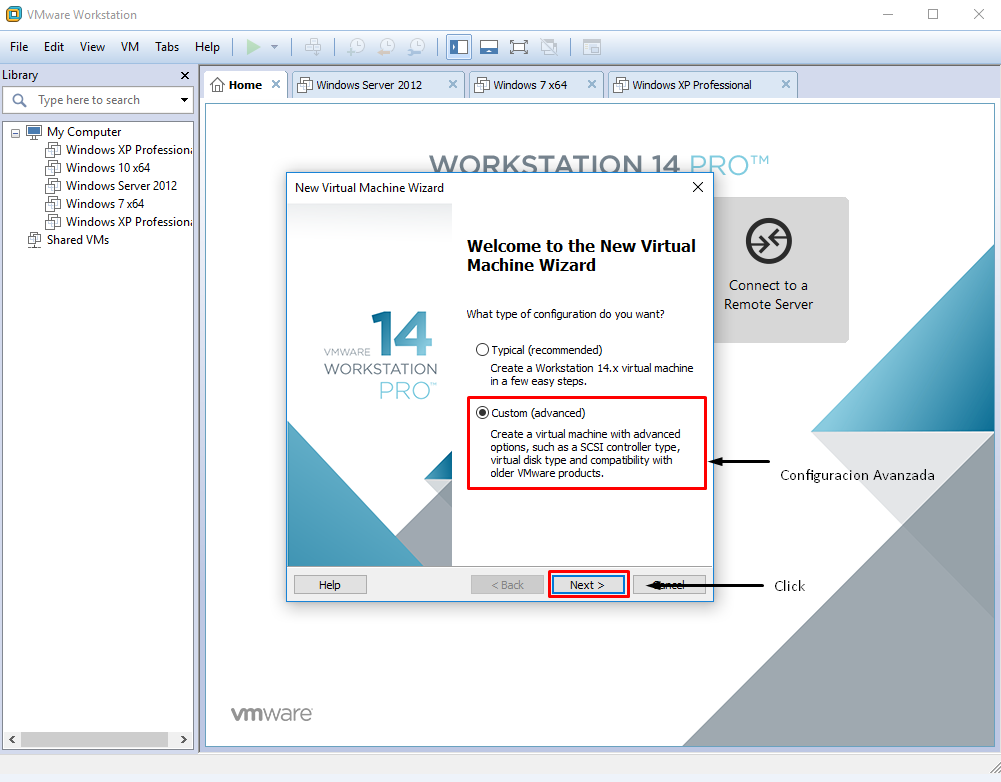
\includegraphics[width=10cm]{./Imagenes/ang1} 
	\end{center}
	

	\item Luego nos aparecera otra ventana en la cual vamos a marcas la tercera opcion la cual indica que instalaremos el ISO despues de la configuracion de la maquina Virtual y le damos en   		\\Next.\\
	\begin{center}
	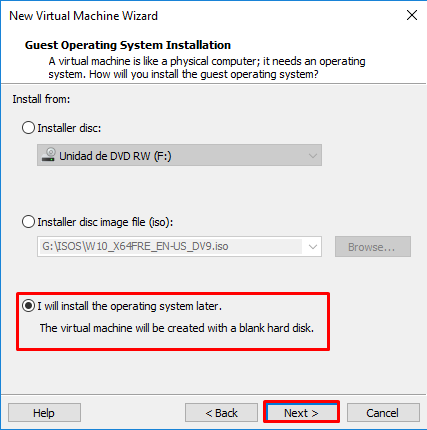
\includegraphics[width=10cm]{./Imagenes/ang2} 
	\end{center}
	
	
	\item Luego tendremos que escoger que sistema operativo vamos a utilizar y su version , como nosotros trabajaremos con Windows Server 2012 R2 tendremos que escoger el Microsoft      		\\Windows y buscaremos el Windows Server 2012 y le damos en Next\\
	\begin{center}
	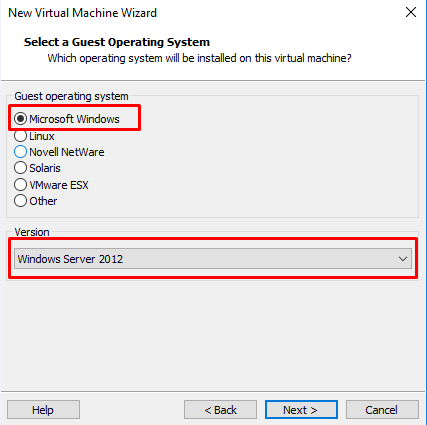
\includegraphics[width=10cm]{./Imagenes/ang3} 
	\end{center}
	

	\item Luego tendremos que rellegar el nombre de la maquina viertual y tambien donde se contrara ubicada nuestra maquina virtual , tener en cuenta que podemos cambiar la ruta de la       		\\ubicacion de la maquina virtual a nuestro gusto. \\
	\begin{center}
	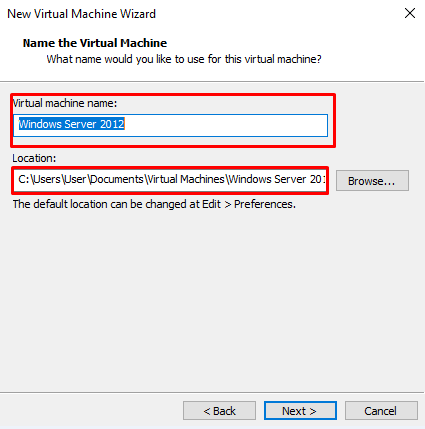
\includegraphics[width=8cm]{./Imagenes/ang4} 
	\end{center}
	

	\item En la siguiente ventana nos aparecera la capacidad de la memoria con la cual trabajara nuestra maquian virtual nosotros lo dejaremos por defecto la recomendada , Luego le damos    		\\en Next.\\
	\begin{center}
	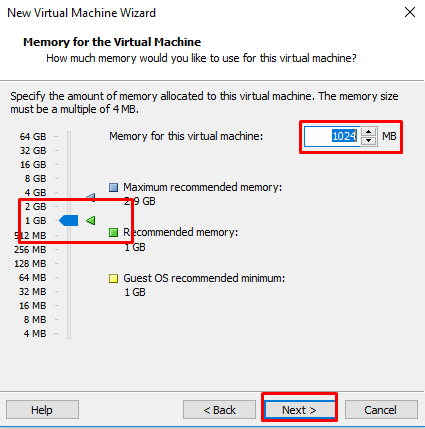
\includegraphics[width=10cm]{./Imagenes/ang5} 
	\end{center}
	

	\item Al Correr la instalacion y despues de poner el ISO del sistemera operativo Windows Server 2012 R2 le daremos en ejecutar y esperamos que cargue la ventana de inicio de nuestro     		\\ISO la cual aparecera , caso contrario revisar el ISO o verificar la configuracion de la maquina virtual , al iniciar el ISO nos aparecera una ventana de inicio en la cual daremos en Install      		\\Now. \\
	\begin{center}
	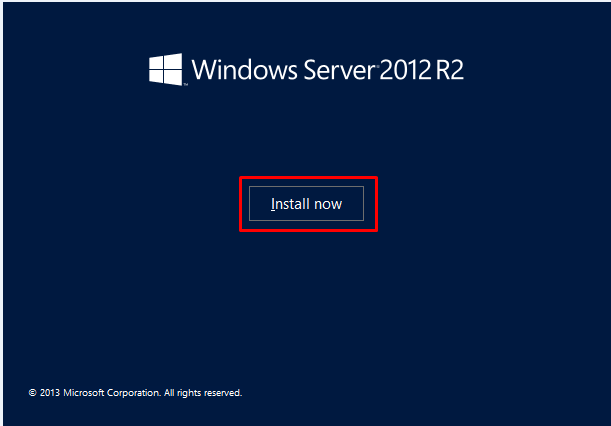
\includegraphics[width=10cm]{./Imagenes/ang6} 
	\end{center}
	

	\item Luego de eso la siguiente ventana sera la configuracion de con la cual trabajara nuestro sistema operativo , para facilitar nuestro proceso de desarrollo escogeremos la interfaz (GUI) 		\\la cual es la recomendad para trabajar mas rapido y eficaz.\\
	\begin{center}
	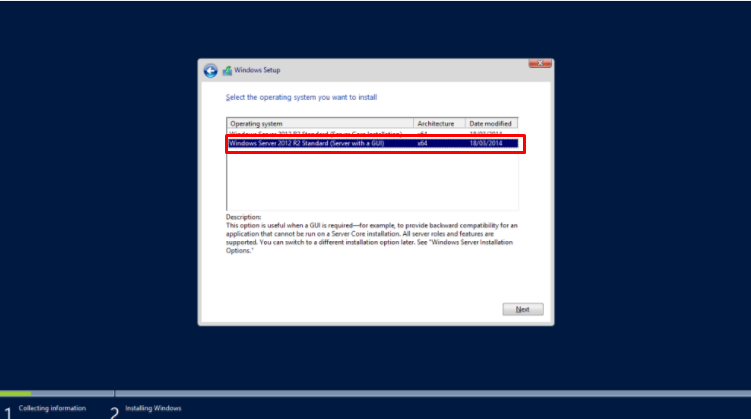
\includegraphics[width=18cm]{./Imagenes/ang7} 
	\end{center}
	


	
\end{enumerate} 
